\chapter{Architektura systemu AVS}
\label{cha:ArchitekturaSystemuAVS}

\begin{figure}[!htb]
	\centering
	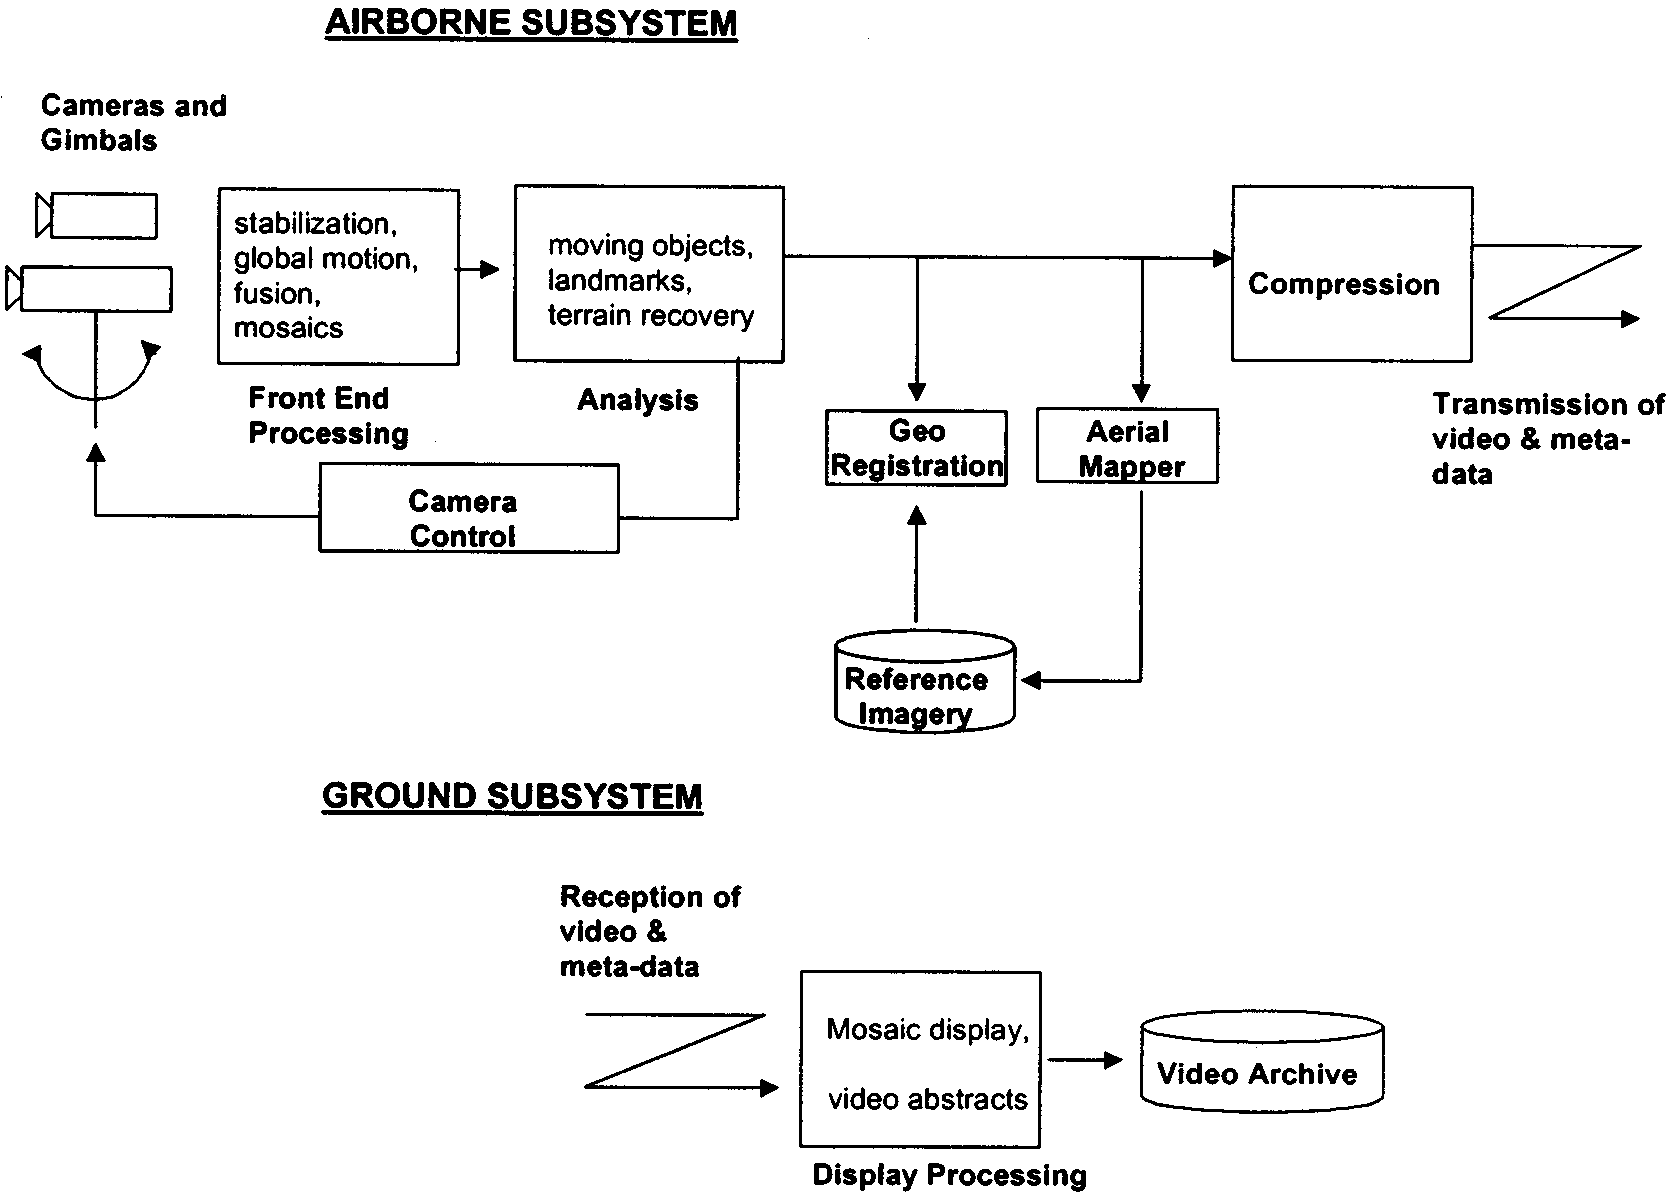
\includegraphics[width=10cm]{Images/AVS_schema_KuSaw01.png} 
	\captionsource{Schemat ideowy systemu AVS do zastosowań w UAV}{\cite{Kumar2001}}
	\label{img:AVS_schema}
\end{figure}

Współczesne systemy AVS umożliwiają automatyczną lub semi-automatyczną obserwację obiektu zainteresowania (zwykle naziemnego), często stanowiąc integralną część systemu sterowania pojazdu UAV, służącego jako platforma operacyjna. 

\section{Elementy składowe}
\label{sec:ElementySkladowe}
\subsection{Kamera wizyjna}
\label{subsec:KameraWizyjna}
Podstawowym źródłem danych wejściowych dla automatycznego systemu AVS jest pojedyncza cyfrowa kamera video. Kamera 


\label{subsec:SensorWizyjny}
Systemy AVS wykorzystywane w pojazdach UAV do rejestrowania obrazu wykorzystują jedną lub dwie kamery video. Kamery video posiadają relatywnie niską rozdzielczość (w porównaniu do aparatów fotograficznych). Dokładna obserwacja obiektu znacznie oddalonego obiektu wymaga w związku z tym zastosowania teleobiektywu - obiektywu o dużej ogniskowej i małym kącie widzenia. W wyniku tego pole widzenia kamery jest niewielkie, przez co konieczne jest jej zorientowanie w kierunku obiektu zainteresowania.  Kamery montowane są na głowicach (\textit{gimbal}) wyposażonych w  stabilizatory oraz mechanizmy \textit{pan-tilt}, których funkcją jest wibroizolacja oraz odpowiednie orientowanie kamery. W niektórych konfiguracjach dodatkowo stosuje się dalmierze laserowe oraz laserowe wskaźniki celu. Aby system działa poprawnie konieczna jest również znajomość pozycji kamery i kalibracja systemu wizyjnego, a więc znajomość meta-danych telemetrycznych, takich jak położenie i orientacja kamery w globalnym układzie współrzędnych oraz jej parametry wewnętrzne - wartość ogniskowej, położenie środka pola widzenia, etc.

\begin{figure}[!htb]
	\centering
	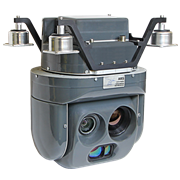
\includegraphics[height=4cm]{Images/ars_tracking_module_wwwuavseu.png} 
	\captionsource{Przykład głowicy do zastosowania w UAV - ARS UAVS Poland}{\url{http://www.uavs.eu/img/products/ars.png}}
	\label{img:ARS_head}
\end{figure}

\subsection{Przetwarzanie obrazu}
\label{subsec:przetwObrazu}
\subsubsection{Przetwarzanie wstępne}
\label{subsubsec:przetwWst}
W pierwszej kolejności obraz zarejestrowany przez kamerę jest poddawany obróbce mającej na celu polepszenie jego jakości oraz przygotowanie do dalszej analizy. Przykładem operacji wykonywanych na obrazie w trakcie przetwarzania wstępnego może być filtracja, mozaikowanie, skalowanie etc.
\subsubsection{Analiza}
\label{subsubsec:analiza}
Wstępnie przetworzony obraz jest następnie poddawany analizie, mającej na celu uzyskanie informacji przydatnej w kontekście funkcji systemu. Może być to na przykład wykrywanie poruszającego się obiektu i śledzenie go pomiędzy kolejnymi klatkami. 

\subsection{Sterowanie kamerą}
Na podstawie danych uzyskanych w wyniku przeprowadzonej analizy przeprowadzane jest odpowiednie sterowanie kamery, w skład którego wchodzi kontrola jej orientacji oraz ewentualne dostrajanie innych parametrów, takich jak długość ogniskowej czy wartość liczby przysłony. Sterowanie ma celu realizację określonej funkcji systemu, jak np. nadążanie kamerą za poruszającym się obiektem, czy skanowanie obserwowanego obszaru.
